\documentclass[10pt,twocolumn]{article}
\usepackage{multicol}
\usepackage{amsmath}
\usepackage{alltt}
\usepackage{framed}
\usepackage{caption}
\usepackage{pdfpages}
\begin{document}

\begin{multicols}{2}
\title{Construction of Story Telling Graphs}
\author{
    Paul C. Nichols\\
    Department of Computer Science\\
    University of California, San Diego\\
    pnichols@cs.ucsd.edu
}
\date{}
\maketitle
\end{multicols}

\begin{abstract}
Stream-like data sources, such as a collection of RSS feeds, can be challenging to summarize as the corpus is ever growing and the nature of the data evolves over time.  This project implements an intelligent RSS reader that leverages topic modeling to provide a high-level view of the document stream.  LDA Topic modeling is performed at daily intervals and linkages between learned topics from different days are computed to form the edges in what can be considered a ``Story Graph".  This story graph can be used to answer a number of contextual questions from both the perspective of a topic and a document.
\end{abstract}

\section{Introduction}
Stream-like data sources are a common fixture of the current technological landscape.  Well known examples of streaming data sources include news content from major media outlets (i.e. through RSS feeds), the collective musings of Twitter's user base  (i.e. the Twitter Firehose), and the click-stream generated from surfing internet (i.e. from network logging).  Summarizing and contextualizing information in a data stream is a natural and important problem that arises.  

The most popular form of summarization on a data stream is mining for trending topics, typically through an unsupervised learning process. Trending topics provide a high level view of the prominent themes present in a data stream during a window of time.  A set of trending topic sets, or even multiple sets from different windows of time, can provide insight in isolation.   However, contextual questions about a topic's origin, lifetime, momentum, and evolution cannot be addressed.  To answer these more advanced questions, topics must be linked beyond the window in time they were discovered.  This set of time sensitive topics and the linkages between them is referred to in this report as a ``Story Graph".  

Given a set of topics, the construction of a story graph is only slightly more complicated than the discovery of the topics themselves.  However, not all approaches to topic discovery result in representations where computing linkages between topics is straight forward.  Further, the topic modeling should be sufficiently powerful to accommodate complicated real-world mixtures of topics.  For both of the above reasons, Latent Dirichlet Allocation (LDA) is used on the bag of word representation of documents to mine for topics. 

Queries on a story graph may start and end from both the perspective of a topic and a document.  Starting from a topic, the story graph can be traced to another topic or down to a document through the topic weights.  Likewise, starting from a document, the story graph can be traced through the topic weights to another topic or again down to a neighboring document.  Features of a trace through the graph, such as the length in time covered or the number of topics or documents traversed, serve as the basis for the answers to the contextual questions posed above.

This project investigates story graphs, their construction process, and their relevant queries by implementing a system that digests a stream of documents exposed from a collection of RSS feeds and generates a summary view of the data through a web portal.  Three different datasets are explored from different categories: General news, Business, and Sports.  Data was collected by the system for 60 days.

\section {Background}
Unsupervised methods for discovery and summarization of a corpus have a rich history rooted in information retrieval.  Before the more abstract task of a topic discovery became widely known, document clustering was a well studied problem.  Document clustering is used to find inter-document similarities and partitions of similar documents in a corpus.   

The vector space representation of a document is a common place to begin document clustering.  The vector space representation of a document holds term counts by assigning a unique dimension to each term that exists in the corpus.  Various term weighting schemes can be applied to the document vectors such as tf-idf weighting.  These schemes enhance the similarity measures by reducing the contribution of unimportant words such as stop words.  Similarity between two documents in vector space can be measured with a geometric interpretation either, by the angle between them (cosign similarity) or the distance apart (euclidean distance).

A good first step towards topic discovery is the K-means algorithm applied to corpus of tf-idf weighted documents in the vector space representation.  K-means attempts to find a partitioning of the corpus into K groups such that the euclidean distance of a cluster's members is minimized.  Iterative refinement from randomly initialized means can be used to approximate this hard problem.  The most highly weighted term indices of the resulting K mean vectors from a clustering job loosely represent the topics present within the corpus.  The approach is advantageous for streaming data because the learned mean vectors can be compared across clustering jobs from different time windows easily (using either cosign similarity or euclidean distance between the means).  The approach is also desirable because it is simple and fast.  However, the technique lacks the richness of topic mixtures by assuming each document can belong to only one mean vector. 

Another early approach that improves upon the vector space representation is Latent Semantic Analysis (LSA).  LSA computes the singular value decomposition of a document-term matrix to find low-rank approximations of the latent document and term matrices.  The resulting matrix factorization has the property that when a pair of documents or a pair of terms are similar, they will be near (using cosign similarity or euclidean distance) in their respective vector spaces.  LSA is good step towards finding a representation that can capture synonymy and polysemy, but is not suitable in the streaming paradigm where the process repeats and regular intervals.  The resulting matrix factorizations are unique to the document-term matrix they were derived from.  There is no straight forward way to compare either the learned term or the document representations from different time windows.

Probabilistic Latent Semantic Analysis (PLSA) addresses the limitations above with LSA by stepping away from the vector space representation of LSA to a probabilistic representation of terms and document.  PLSA represents documents in the bag-of-word format where term frequency is maintained but not order and no geometric interpretation is applied. PLSA introduces a hidden random variable to model topics and then learns document-topic and topic-term distributions through the Expectation Maximization (EM) algorithm.  PLSA can also overcome issues such as synonymy and polysemy through the topic, and has the advantage of allowing mixtures of topic (or cluster) assignments.  Lastly, PLSA is advantageous in the streaming paradigm because the resulting topic distributions are interpretable and comparable across different time windows. 

PLSA is the predecessor to LDA, the model used in this project.  LDA improves upon PLSA by modeling the document probabilities and word distributions as dependent on Dirichlet prior distributions.  This dependence on prior distributions enhances the generality of the distributions learned.  An LDA model is more complicated and the distributions are commonly estimated using Gibbs Sampling.

\section {Method}
\subsection {Graph Creation}
The starting point of graph creation is corpus of documents partitioned by a time interval over an indefinite period.   Formally, we may represent this by the following notation where the maximum interval $T$ is ever increasing.  

\begin{align*}
\mathbf{C} &= \{ \mathbf{C}_0, \dots, \mathbf{C}_T \} \\
\mathbf{C}_t &= \{\mathbf{d}_0^t, \dots, \mathbf{d}_N^t \} \\
\mathbf{d}_i^t &= \{ w_{i,0}, \dots, w_{i,M} \}
\end{align*}

For the purposes of this project, the partitions $\mathbf{C}_t$ for $t \le T$ represent the documents partitioned by day.  Each individual day's sub-corpus $\mathbf{C}_t$ is a collection documents where each document $\mathbf{d}_i^t$ is in the bag-of-word format.  For the purposes of this document, superscripts are used to denote documents, topics, and distributions from a given day $t$ except when describing running times.  In this project LDA topic modeling is used to estimate from the daily corpus $\mathbf{C}_t$ the probability distributions of the the document-topic distribution, $\theta_{i,k}^t$, and topic-term distribution, $\phi_{j,k}^t$.

\begin{center}
\begin{tabular}{|l|l|}
  \hline
  \multicolumn{2}{|c|}{Summary of LDA Variables} \\
  \hline
  $i < N$ & Number of Documents \\
  $j < M$ & Number of Terms \\
  $k < K$ & Number of Topics \\
  $w_{i, j}$ & Count of Term=j in Document=i \\
  $z_k$ & Topic k of K \\
  \emph{$\alpha_k$} & Document-Topic Prior Parameter\\
  \emph{$\beta_j$} & Topic-Term Prior Parameter \\
  $\theta_{i,k}$ & P(Topic=$z_k$ $\vert$ Document=i) \\
  $\phi_{k,j}$ & P(Word=j $\vert$ Topic=$z_k$) \\
  \hline
\end{tabular}
\end{center} 

The story graph constructed from the learned distributions follows the standard form: $\mathbf{G}$ = $(\mathbf{V}, \mathbf{E})$.  A unique feature of the story graph is that the vertices in $\mathbf{V}$ can include both the documents and the topics and follows directly from the conditional dependence graph of the LDA model.  The edges in $\mathbf{E}$ are undirected, as opposed to directed when representing conditional independence, so traversals in either direction may be performed.  

\begin{figure}[htp] \centering{
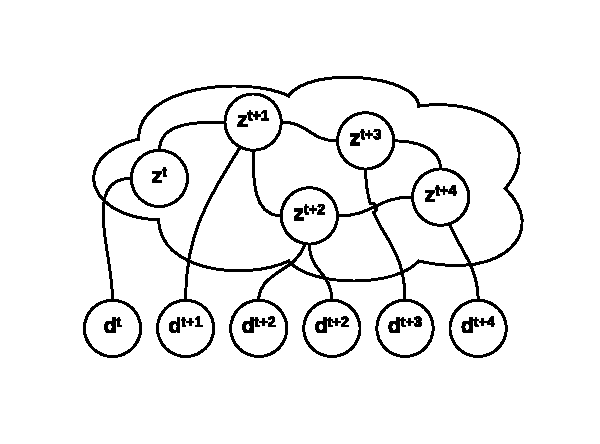
\includegraphics[scale=0.82]{img/story-graph.pdf}}
\caption{Story Graph: An example graph over $t$ to $t+4$ days}
\end{figure}  

Edges and weighted by floating point values ranging between between $[0, 1]$.  Edges between documents are always 0 (i.e. are not allowed).  Topics may form edges with documents of the same day using the document-topic distribution.  Edges between topics across different days are formed by computing the cosign similarity on the vector space interpretation of the topic-word distributions.  Though blatantly not probabilistic, the cosign similarity between two probability distributions will at least always return a value between $[0,1]$. These topic-topic edges are precomputed between the current days topics and all previous days topic within some limit (in this project, 15 days).  The formal rules for constructing edge weights are as follows:  

\begin{align*}
  e(\mathbf{d}_i^t, \mathbf{d}_{i'}^{t'}) &= \quad 0 \qquad\quad \forall \quad i, t, i', t'\\
  e(\mathbf{z}_k^t, \mathbf{z}_{k'}^{t'}) &= \begin{cases}
      0 & \text{if $t=t'$} \\
      \frac{\phi_k^t \cdot \phi_{k'}^{t'}}{||\phi_k^t||\,||\phi_{k'}^{t'}||} & \text{if $t \ne t'$}
    \end{cases} \\
  e(\mathbf{d}_i^t, \mathbf{z}_{k}^{t'}) &= \begin{cases}
      \theta_{i,k}^t & \qquad\quad \text{if $t =t'$} \\
      0 & \qquad\quad \text{if $t \ne t'$}
    \end{cases}
\end{align*}

\subsection {Query by Topic}

Starting from a topic $\mathbf{z_k^t}$, a natural query is to find the sub-graph of related topics across all time.  This sub-graph can be thought of as the story a topic belongs to.  This query performs a breadth first search of the neighboring topics from different days while the product of the edge weights along each path from starting to ending topic is above a threshold between [0,1].   

\begin{framed}
\begin{center}
\begin{alltt}
Define: Subgraph()
Input:  Starting topic \(z\sb{k}\sp{t}\), 
        Topic threshold \(thresh\sb{z}\)
Output: Related topic set \(Z\)
Begin:
  Initialize \(Z = \{\}\),             
             \(V = \{z\sb{k}\sp{t}\}\),
             \(F = \{<z\sb{k}\sp{t}, 1>\}\)
  While \(F \ne \{\}\):
     Remove \(z\) from \(F\)
     For \(z' \in\) TopicNeighbors(\(z\)):
       Let \(w = \)e(\(z, z'\))*weight(\(z\))
       If \(z' \not\in\ V\) and \(w >thresh\sb{z}\):
         \(Z = Z \bigcup <z', w>\)
         \(F = F \bigcup <z', w> \)
     \(V = V \bigcup z\)
  return \(Z\)
End
\end{alltt}
\captionof{alltt}{Algorithm topic sub-graph of topic $z_k^t$}
\end{center}
\end{framed}

Querying the graph for a topic's sub-graph can, in the worse case, be somewhat expensive for long-lived stories.  Breadth first search has a running time in the general case of $O(|E|)$.  For a given day, there will be $K^2W$ edges where $K$ is the number of topics and $W$ is the number of days compared.  A long lived story can trace through $T$ days.  Therefore, the number of edges is $O(TK^2W)$, which is less than the possible $O(T^2K^2)$ edges if windowing were not applied.  Better yet, the edges are pre-computed and only edges above the threshold are added. Typically much less than $K^2W$ edges per day are used in this query.

\subsection {Query by Document}
Another useful query on the story graph is the more classic problem of finding relevant neighboring documents given a starting document.  Again a breadth first search is required.  Recall that documents are connected to the graph only through their topic weights and that the interior of the graph is entirely edges between topics of different days.  Therefore, the traversal of the graph from one document to another may reuse the \texttt{Subgraph()} routine presented in the previous subsection.

A similar approach is taken to querying by document as by topic in that again the paths from document to document will be pruned by the product of the edge weights. To make the algorithm more efficient, a modified version of the \texttt{Subgraph()} routine is assumed where a set of starting topics can be supplied instead of only a single one.  This modification does not change the algorithm or the running time.

\begin{framed}
\begin{center}
\begin{alltt}
Define: Similar()
Input:  Starting document \(d\sb{i}\sp{t}\), 
        Topic-topic threshold \(thresh\sb{z}\),
        Document-topic threshold \(thresh\sb{d}\)
Output: Related document set \(D\)
Begin:
  Initialize \(D = \{\}\),             
             \(F = \{\}\)
  For \(z \in\) TopicNeighbors(\(d\sb{i}\sp{t}\)):
    If e(\(d\sb{i}\sp{t}, z\)) \(> thresh\sb{d}\):
      \(F = F \bigcup <z, 1>\)

  For \(z \in\) Subgraph(\(F, thresh\sb{z}\)):
    For \(d \in\) DocumentNeighbors(\(z\)):
      Let \(w = \)e(\(d, z\))*weight(\(z\))
      If \(w\) \(> thresh\sb{d}\):
        \(D = D \bigcup <d, z, w>\)
  Return \(D\)
End
\end{alltt}
\captionof{alltt}{Algorithm for relevant documents $d_i^t$}
\end{center}
\end{framed}

An interesting consequence of querying by document is that a document may be similar to another document indirectly through multiple topics. The indirect nature of the query makes the running time of the algorithm slower than querying by document.  For a given day $t$, the number of documents retrieved by any topic can be at most the number of documents that day $|\mathbf{C}^t|$.  Therefore, over all time and all topic-topic edges, a factor of $|\mathbf{C}|$ extra edges between documents need be explored.  The total running time is $O(TK^2W|C|)$.  Again, thresholds can be performed prior to updating the graph so many of the total possible edges do not exist.
  
\subsection {Graph Metrics}

Given a topic's sub-graph, there are a number of interesting metrics that can be used to analyze the story. The first query of interest is the lifetime of a story.  The lifetime of a story is simply the maximum topic time window less the minimum.  Knowing the total time a story has existed can then be used to estimate what can be interpreted as density or velocity.  Story density or velocity is defined as the number of topics in the subgraph divided by a time range.  This time range can be the lifetime if examining a story in isolation or an arbitrary range if comparing multiple stories.  

The number of documents a given topic connects to in the sub-graph provides a notion of size.  A threshold is required to ensure documents are truly relevant to the topic, which is described in the next section.  The number of relevant documents over an entire subgraph can be thought of as the story's mass. Putting the velocity and mass together, the notion of momentum can be borrowed from physics to assess how enduring a story is. 

An alternative measure of size of a topic is the hyper-parameter $\alpha_k$.  In previous versions of LDA this parameter had to supplied, but now can be estimated from the corpus using a burning period.  The topic modeling software used in the project performs this estimation.

For notation, let $\mathbf{S}$ be a topic's sub-graph and let $\mathbf{D}_\mathbf{S}$ be the number of unique documents connected to the sub-graph with a path product above the threshold used in \texttt{Similar}().  The various metrics are stated below in these terms.

\begin{align}
\texttt{Lifetime}(\mathbf{S}) &=\max_{z \in \mathbf{S}} \texttt{time}(z) - \min_{z \in \mathbf{S}}\texttt{time}(z) \\
\texttt{Velocity}(\mathbf{S}) &= \frac{|\mathbf{S}|}{\Delta \text{time}} \\
\texttt{Mass}(\mathbf{S}) & = |\mathbf{D}_\mathbf{S}| \\
\texttt{Mass2}(\mathbf{S}) & = \sum_{z \in \mathbf{S}} \alpha_z\\
\texttt{Momentum}(\mathbf{S}) &= \texttt{Mass}(\mathbf{S}) \times \texttt{Velocity}(\mathbf{S})
\end{align}

\section {Architecture}

Processing the document stream is accomplished by a nightly process that downloads content from a collection of RSS feeds for the previous day.  The entire process is composed a series of stages that happen sequentially.  While the production environment schedules the process to handle a single day's worth of data from a cron job, the process can also be run in batch mode to process all data over a provided time range.  Importantly, each stage in the processing pipeline is dependent only on the output from the previous stage.

The process begins with the sync stage by gathering the list of URLs for unprocessed data in the stream using the Google Reader undocumented API (GRAPI).  The GRAPI normalizes the many quirks and formatting issues present in a large set of RSS/Atom feeds and exposes a standard representation of a document stream.  The output of the Sync stage is a mapping for URL to path on local storage the content should be downloaded to.

The fetch stage of the processing pipeline is run after the Sync stage generates output.  This stage is responsible for downloading HTML content, extracting the relevant article content from the raw HTML, and saving the result to local disk.  Content downloading is managed by through the Apache Commons libraries.  Article extraction was originally handled by extracting text content with an HTML parser.  However, the resulting saved documents included too many artifacts of the hosting site such as advertisements, comments, and boiler plate content.  The artifacts present in the document made the topic modeling perform poorly.  To remedy this problem, a library known as ``boilerpipe`" was used to separate article content from artifact with an in-built decision tree classifier.

The next stage of the pipeline performs topic modeling on the daily corpus that was created locally from the Fetch stage.  Topic modeling is handled by the ParallelTopicModel in the Mallet library.  Documents are transformed into the bag-of-word format by converting characters to lower case, removing punctuation, and splitting on whitespace.  A burn-in phase of 10 iterations is used to estimate the Dirichlet hyper-parameters. The learned topics improve qualitatively when the content is boosted by appending the a document's title 5 times.  The number of topics, K, is chosen to be half the corpus size.  This allows space for redundant themes to cluster on a single topic, but also the common situation where a topic has no history and is new or one-time event.

\begin{figure}[htp] \centering{
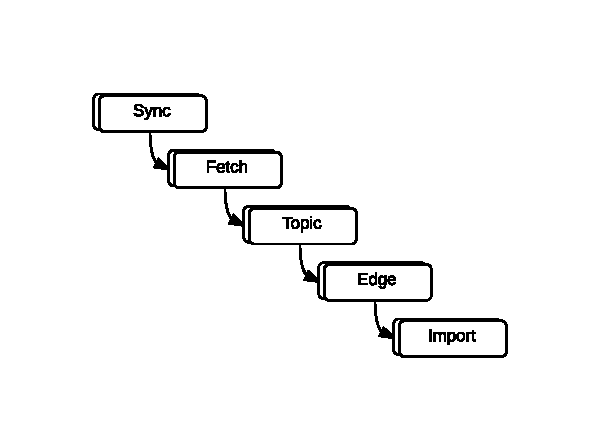
\includegraphics[scale=0.82]{img/system-diagram.pdf}}
\caption{Architecture Diagram: Sequential Stages}
\end{figure}  

After the topic modeling has completed for the current day, edges are computed between topics of the previous days within a given window of time.  As time progresses, the total time frame a similar topic can be detected is the window of days before and after the topic date.  Similarity between topics is computed by treating the topic-term distribution as a vector space representation and computing the cosign-similarity.  

Lastly, after all the previous stages have completed the downloaded document data, topic distributions, and similarity measures are imported into a database.  After the import process completes the max date is updated so that queries may be performed agains the new, fully imported day's worth of information.  The database contains all information required by the web portal to let a user explore the data stream and answer relevant story graph queries.


\section {Evaluation}

\subsection {Popular Topics}
Does the topic modeling work? Show samples of popular learned topics.  Possibly show impact of boosting, extraction.

\subsection {Topic Topic Edges}
Does the edge creation work?  Show samples of topic-topic edges and histogram of typical edge weight to estimate branch factor.  Discuss threshold setting.

\subsection {Topic Metrics}
How useful are topic metrics? Show samples/summary plots of topic lifetime, velocity, and momentum

\subsection {Document Topic Edges}
Can the story graph find relevant document given a starting document.

\section {Future Work}

\end{document}
